\makeatletter
\def\input@path{{../../tex/}{../another-directory/}}
\makeatother

\documentclass[aspectratio=169]{beamer}

% Document metadata
\title{ExaMA}
\subtitle{Methods and Algorithms at ExaScale}
\author[CP/HB]{Christophe Prud'homme \& Hélène Barucq}
\institute{}
\date{\today}

% Image for the title page (use includegraphics option to properly size/place it)
\titlegraphic{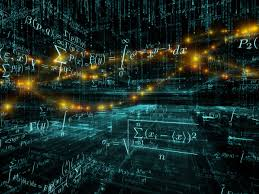
\includegraphics[height=\paperheight]{../../figures/math-hpc.jpeg}}

\usetheme[sectionstyle=style2]{trigon}

% Define logos to use (comment if no logo)
\biglogo{../../figures/exascale.png} % Used on titlepage only
\smalllogo{../../figures/exascale.png} % Used on top right corner of regular frames

% ------ If you want to change the theme default colors, do it here ------
%\definecolor{tPrim}{HTML}{00843B}   % Green
%\definecolor{tSec}{HTML}{289B38}    % Green light
%\definecolor{tAccent}{HTML}{F07F3C} % Orange

% ------ Packages and definitions used for this demo. Can be removed ------
\usepackage{appendixnumberbeamer} % To use \appendix command
\pdfstringdefDisableCommands{% Fix hyperref translate warning with \appendix
\def\translate#1{#1}%
}
\usepackage{pgf-pie} % For pie charts
\usepackage{caption} % For subfigures
\usepackage{subcaption} % For subfigures
\usepackage{xspace}
\newcommand{\themename}{\textbf{\textsc{trigon}}\xspace}
\usepackage[scale=2]{ccicons} % Icons for CC-BY-SA
\usepackage{booktabs} % Better tables

%==============================================================================
%                               BEGIN DOCUMENT
%==============================================================================
\begin{document}

% !TEX root=exama-221018.tex
%--------------------------------------
% Create title frame
\titleframe

%--------------------------------------
% Table of contents
\begin{frame}{Overview}
  \setbeamertemplate{section in toc}[sections numbered]
  \tableofcontents[hideallsubsections]
\end{frame}


%==============================================
\section{PEPR NumPEX}

\subsection*{NumPEX}
\begin{frame}
  \frametitle{\insertsectionhead}
  \framesubtitle{\insertsubsectionhead}
\footnotesize
  \begin{columns}
    \begin{column}{0.5\textwidth}
      \begin{itemize}
        \item \alert{Aggregate the French HPC/HPDA/IA}
        community
        \item Contribute and accelerate the emergence of a 
        \alert{European sovereign exascale software stack and strategic applications exascale capability in a coherent and multi-annual framework}
        \item Integrate and validate \alert{co-designed} innovative methods, libraries and software stack with demonstrators of strategic applications.
        \item Accelerate science-driven and engineering-driven developers \alert{training and software  productivity}
      \end{itemize}
    \end{column}
    \begin{column}{.5\textwidth}
      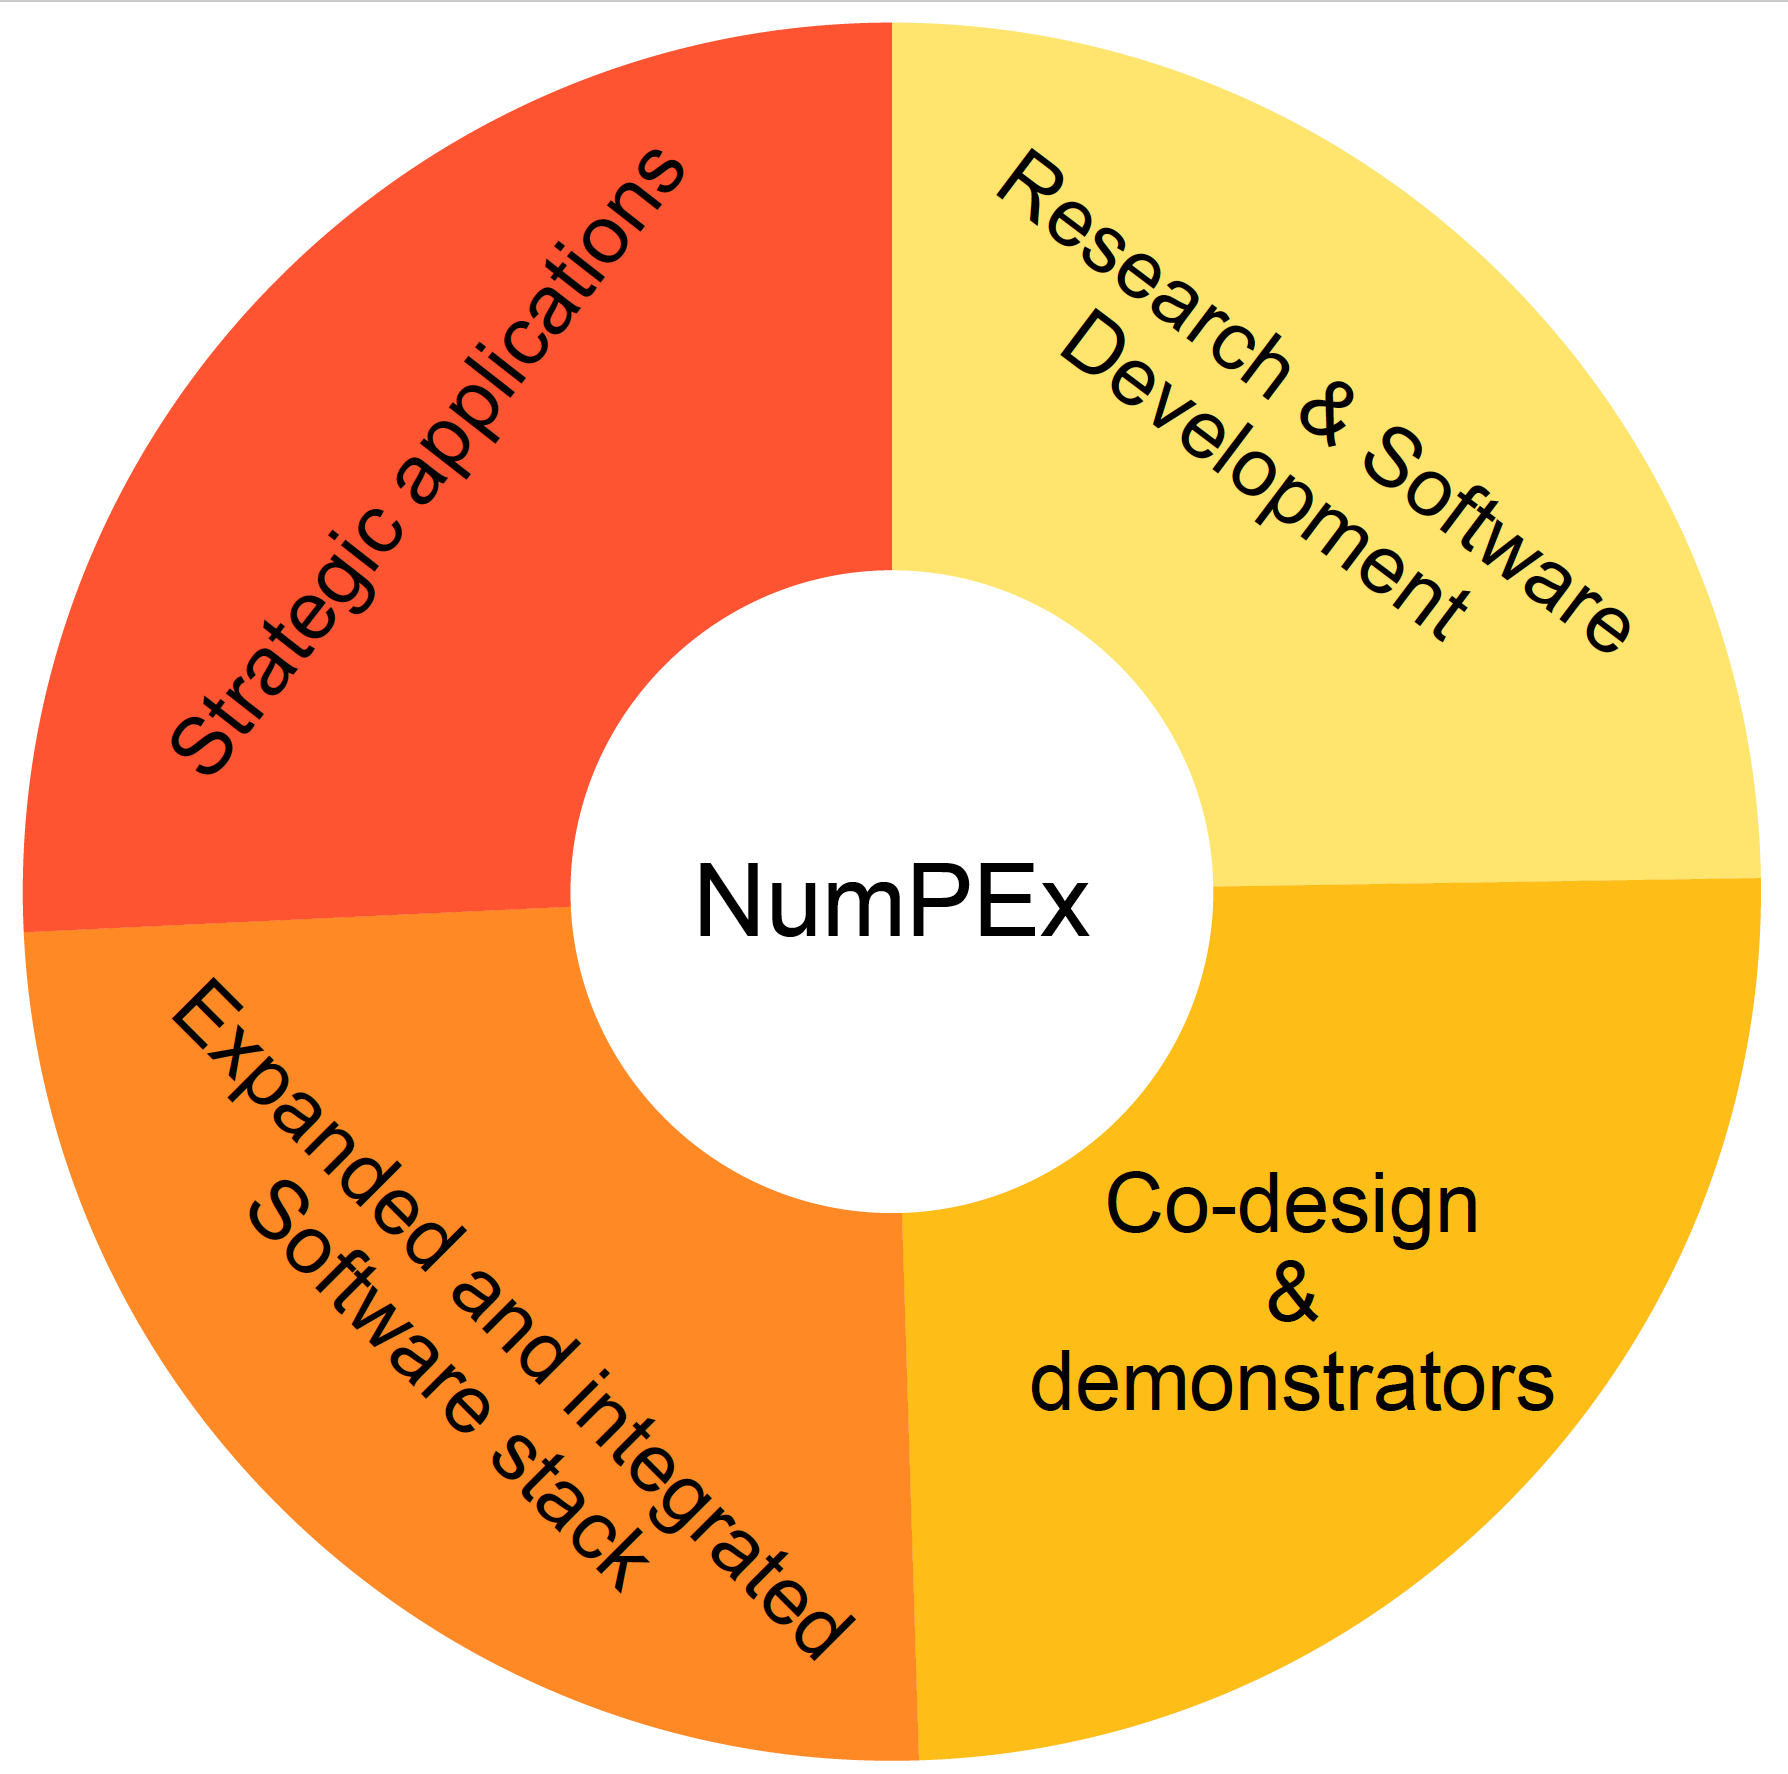
\includegraphics[width=\textwidth]{../figures/numpex-objectives.png}
    \end{column}
  \end{columns}

\end{frame}

\subsection{NumPEx::PC123}

\begin{frame}
  \frametitle{\insertsectionhead}
  \framesubtitle{\insertsubsectionhead}
  \begin{columns}
    \begin{column}{0.5\textwidth}
      \begin{alertblock}{PC<n>\footnote{PC Projet ciblé $\equiv$ IP Integrated project}}

      \begin{enumerate}
        \item \alert{PC1} \textbf{Methods and algorithms for
        Exascale}
        \item \alert{PC2} \textbf{HPC software and tools for the
        Exascale}
        \item \alert{PC3} \textbf{Data-oriented software and tools
        for the Exascale}
      \end{enumerate}
              
    \end{alertblock}
    \end{column}
    \begin{column}{.5\textwidth}
      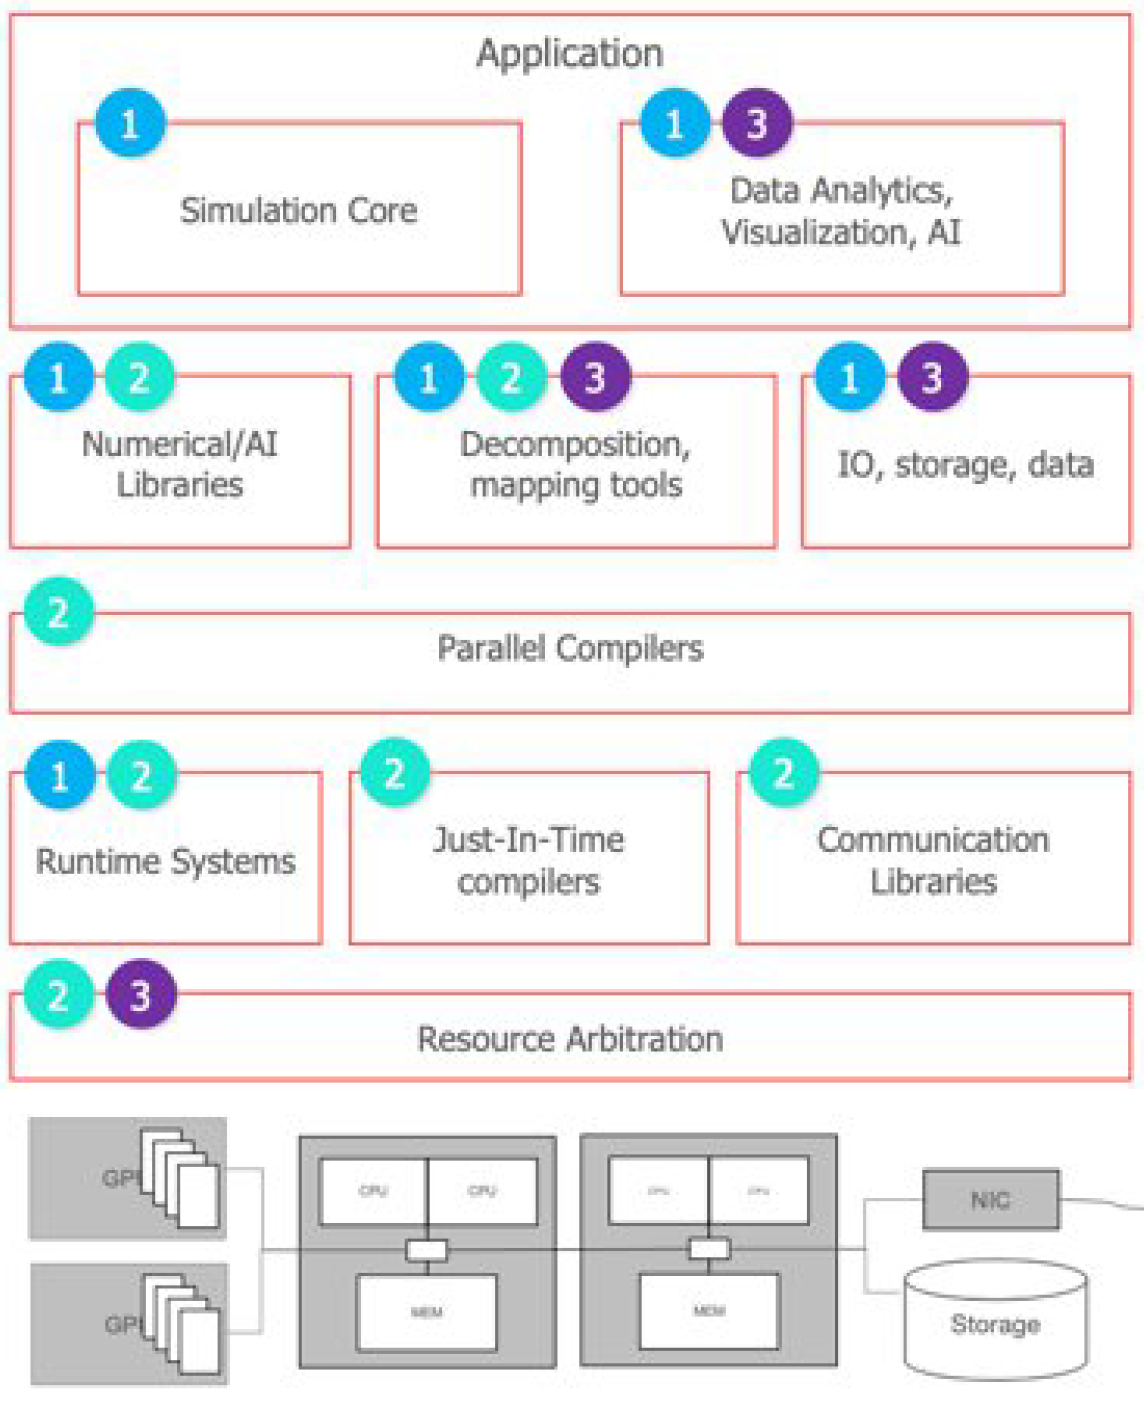
\includegraphics[height=.76\paperheight]{../figures/numpex-ip123.png}
    \end{column}
  \end{columns}
  
\end{frame}
\subsection{NumPEx::PC4}

\begin{frame}
  \frametitle{\insertsectionhead}
  \framesubtitle{\insertsubsectionhead}

  \begin{columns}
    \begin{column}{0.5\textwidth}
      \begin{alertblock}{Wide-area exascale workflows and
        architecture}
        \begin{itemize}
          \item Data logistic between data sources
          (e.g. large scientific instruments) and
          the Exascale system
          \item Cybersecurity and environmental
          sustainability focus
          \item Promoting EU technology (e.g. Atos
          data node and edge servers)
        \end{itemize}
      \end{alertblock}
      
    \end{column}
    \begin{column}{.5\textwidth}
      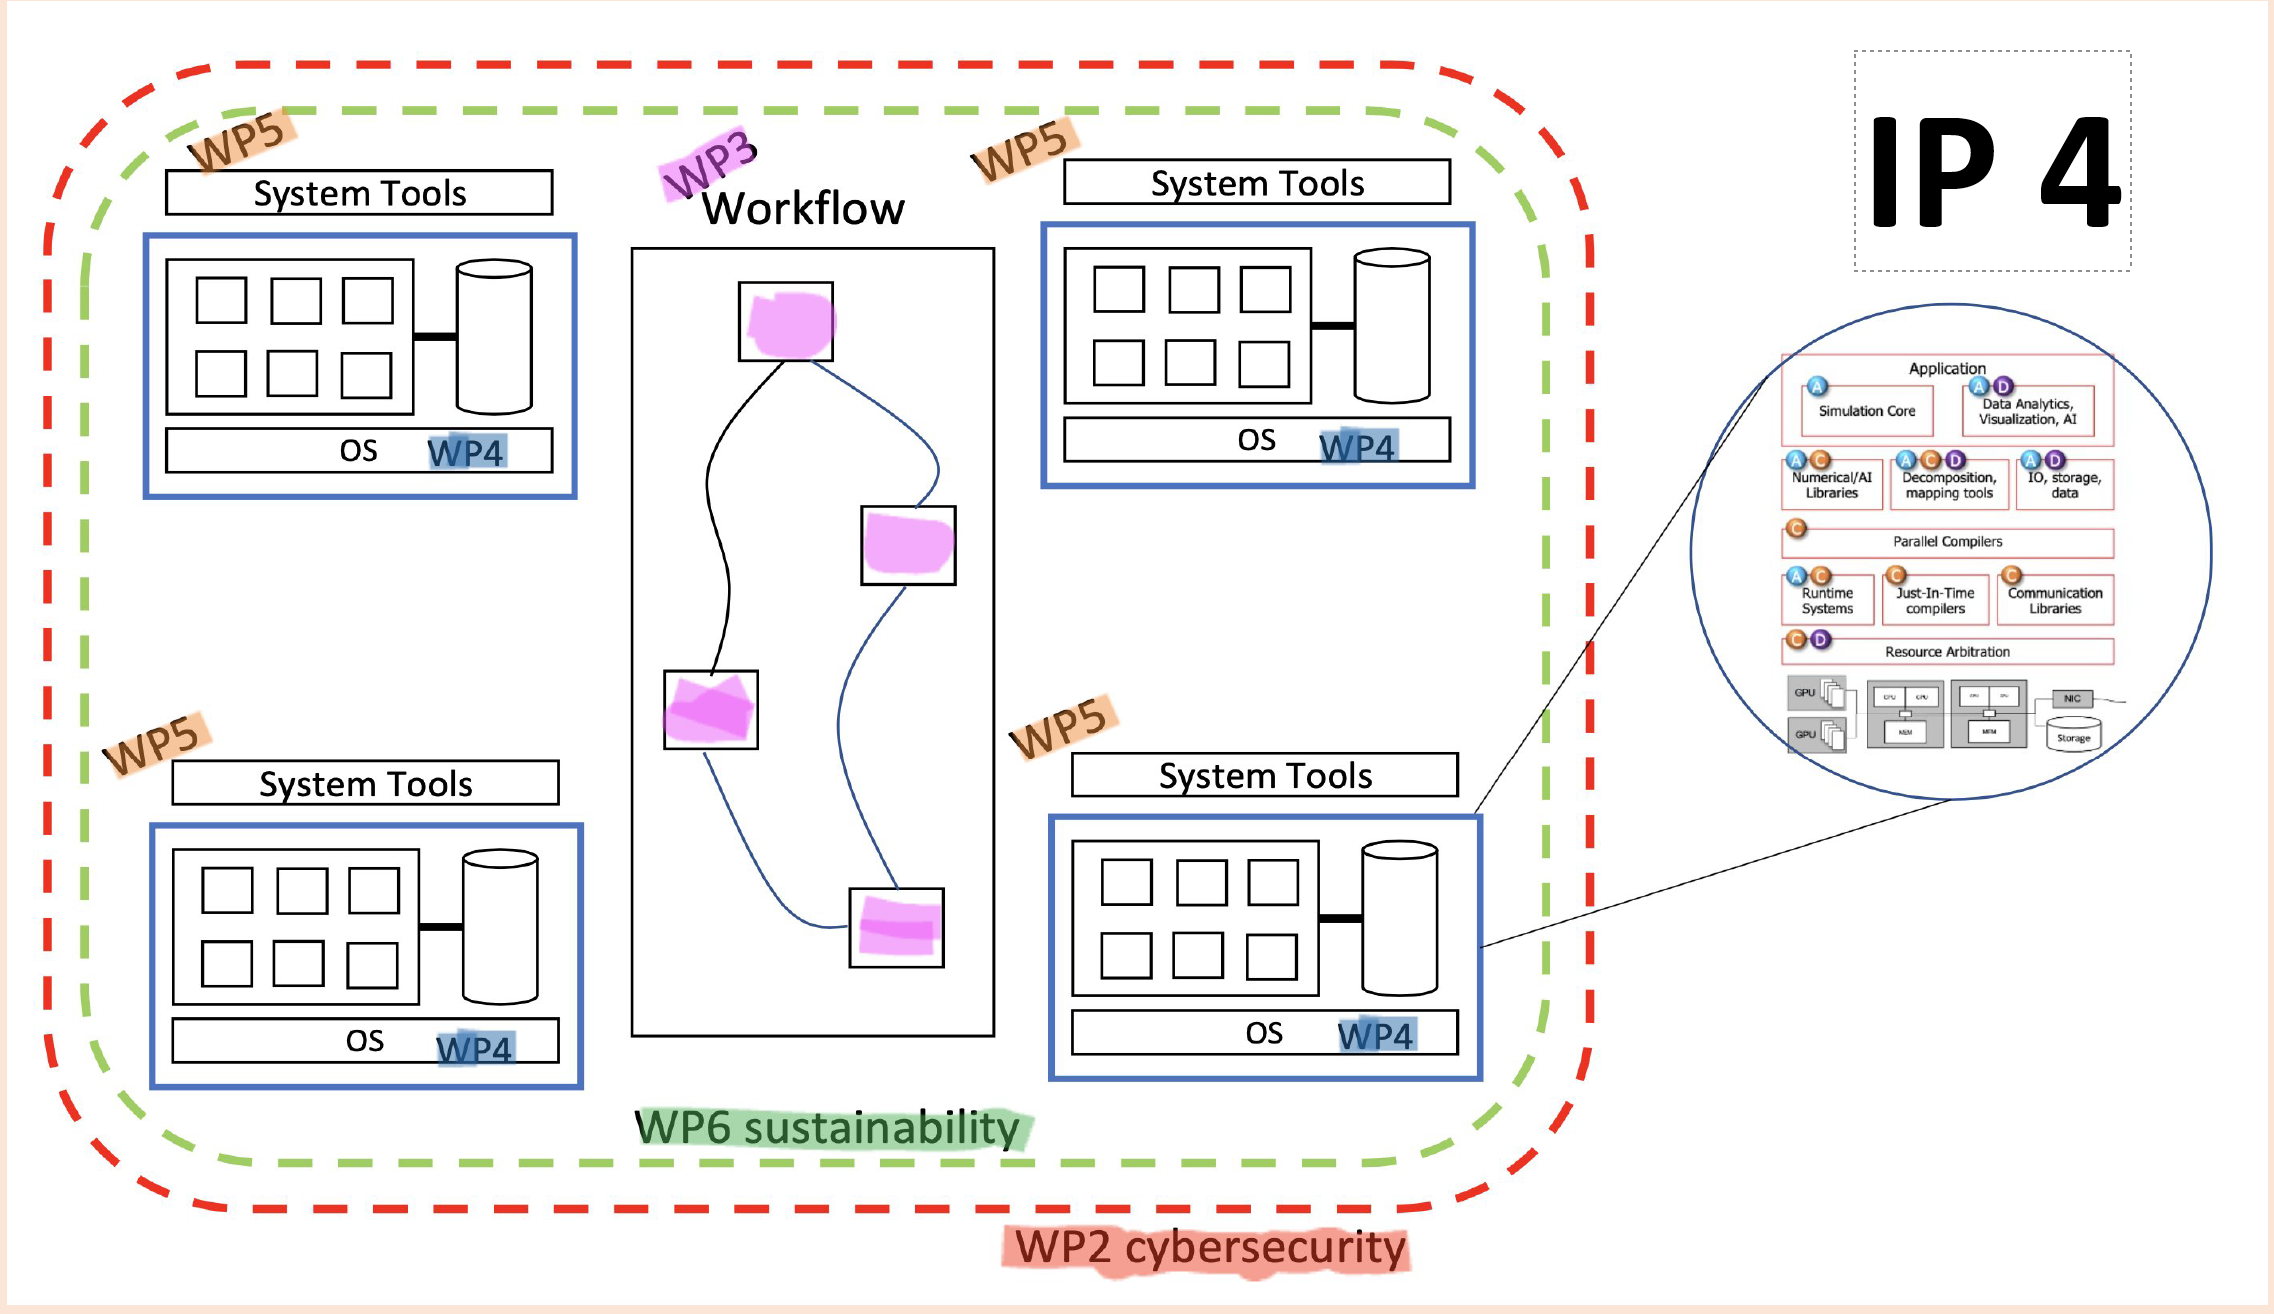
\includegraphics[width=\textwidth]{../figures/numpex-ip4.png}
    \end{column}
  \end{columns}

\end{frame}


\subsection{NumPEx::PC5}

\begin{frame}
  \frametitle{\insertsectionhead}
  \framesubtitle{\insertsubsectionhead}
  \begin{columns}
    \begin{column}{0.5\textwidth}
      \begin{alertblock}{IP 5: Co-design development, software productivity, and demonstrators}
      \begin{itemize}
        \item Identify and define co-design motifs across domain demonstrators and NumPeX
        \item Push R\&D demonstrators requirements into software R\&D (IP 1-4)
        \item Push integrated software developments into demonstrators      
      \end{itemize}
      \end{alertblock}
    \end{column}
    \begin{column}{.5\textwidth}
      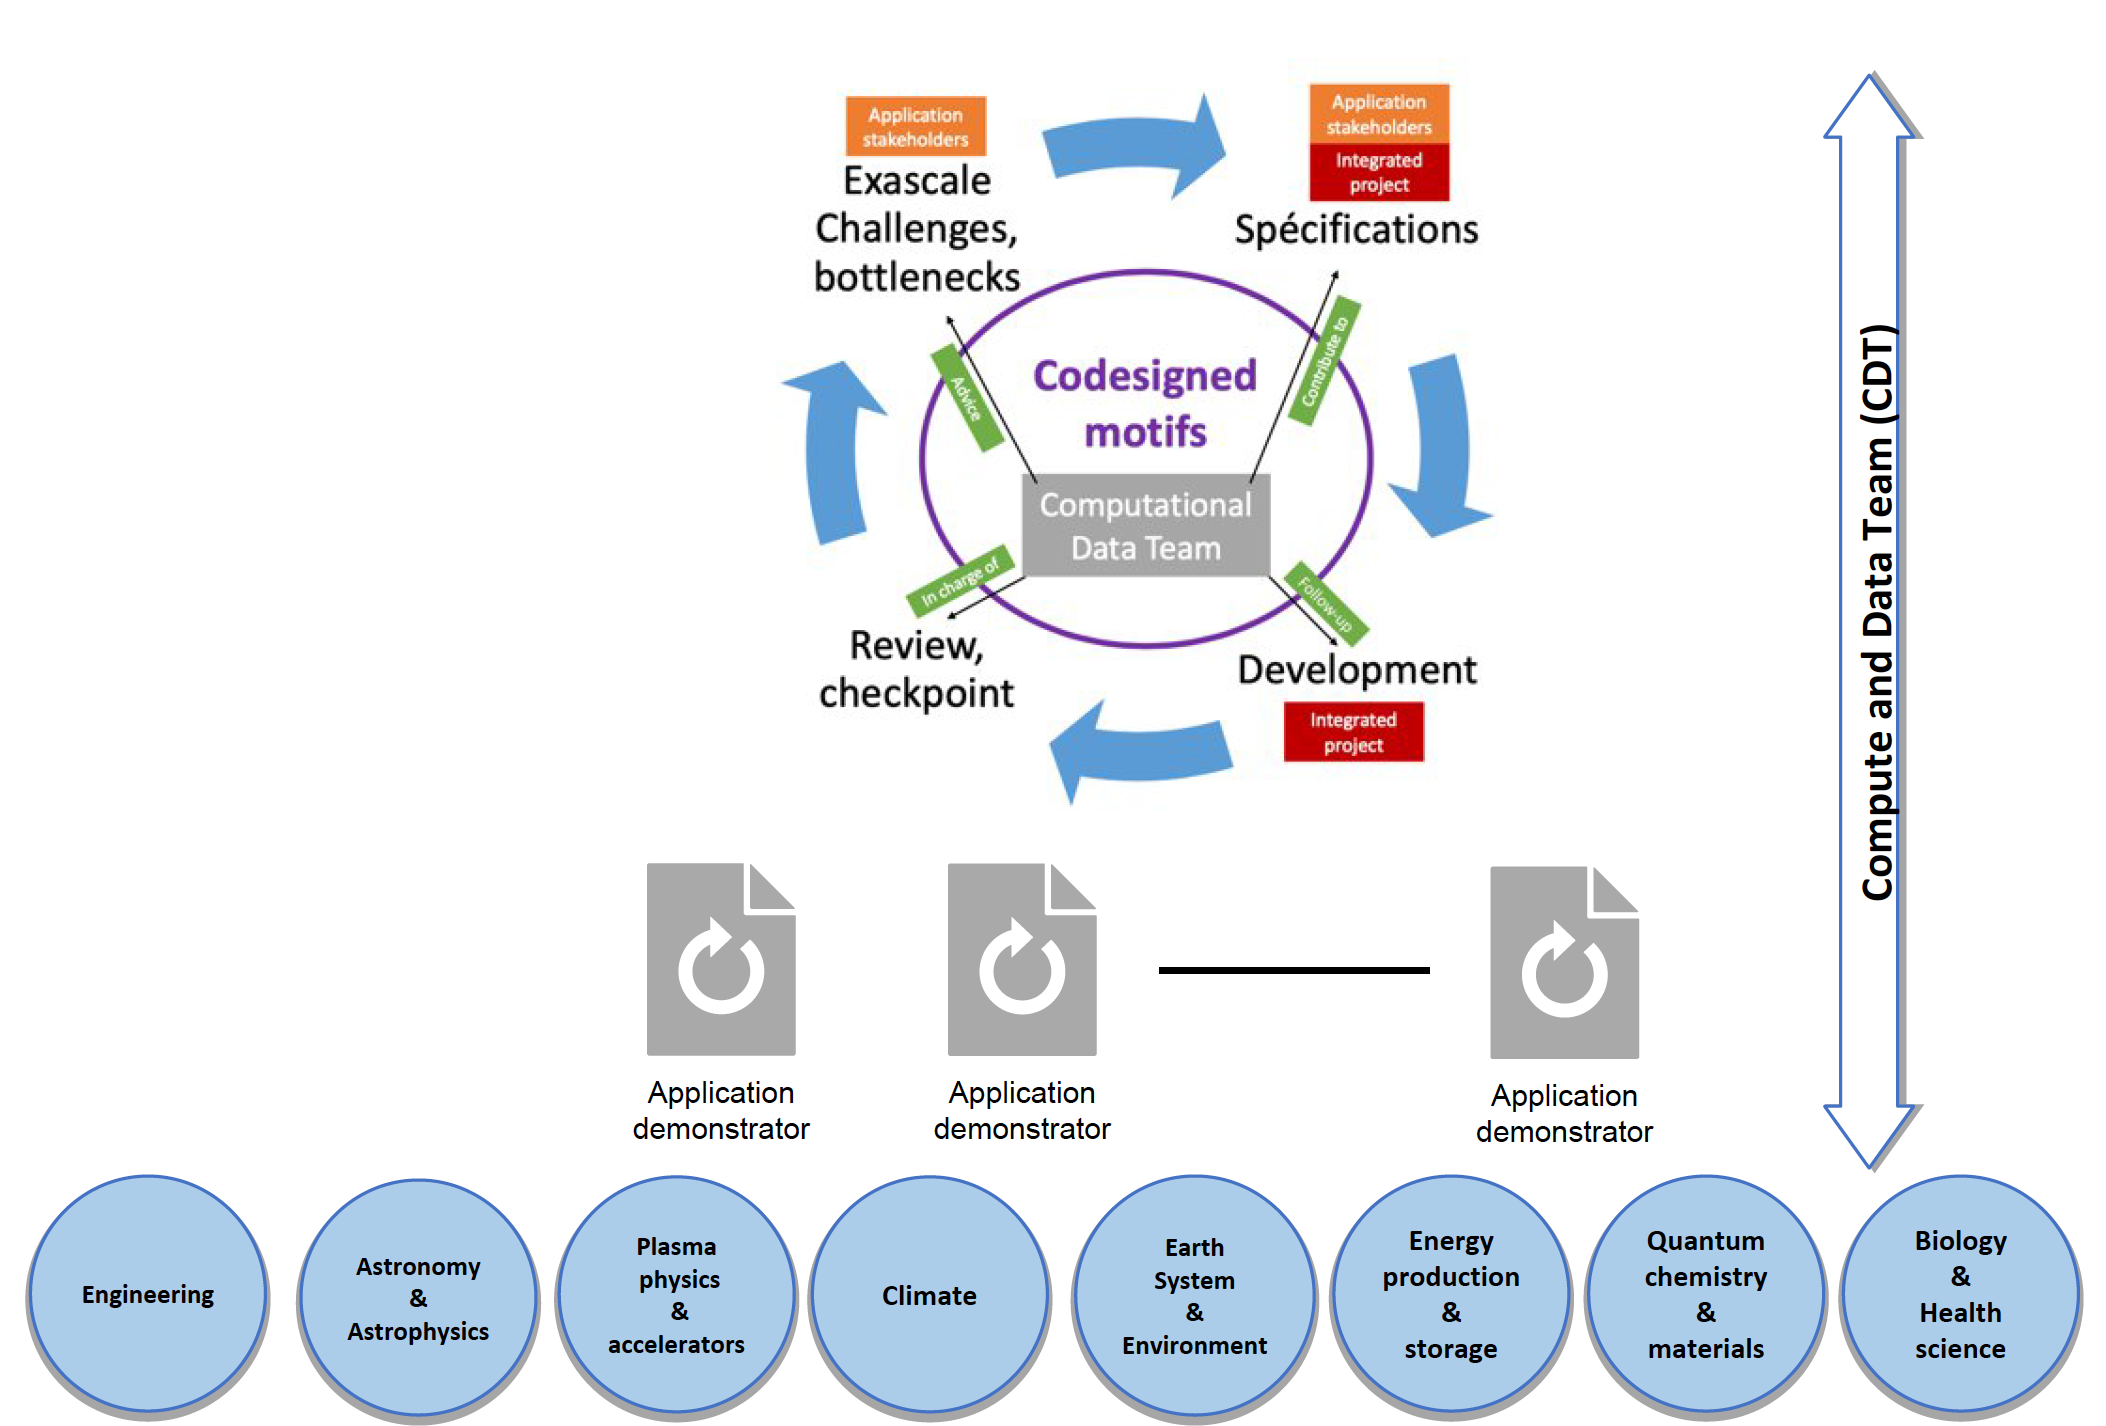
\includegraphics[width=\textwidth]{../figures/numpex-ip5-2.png}
    \end{column}
  
  \end{columns}
\end{frame}
\subsection{NumPEx::Software Integration and Productivity}
\begin{frame}
  \frametitle{\insertsectionhead}
  \framesubtitle{\insertsubsectionhead}

  \begin{columns}[t]
    \begin{column}{.5\textwidth}
       \begin{figure}[ht]%
         \centering
          \begin{subfigure}{.45\textwidth}\centering
            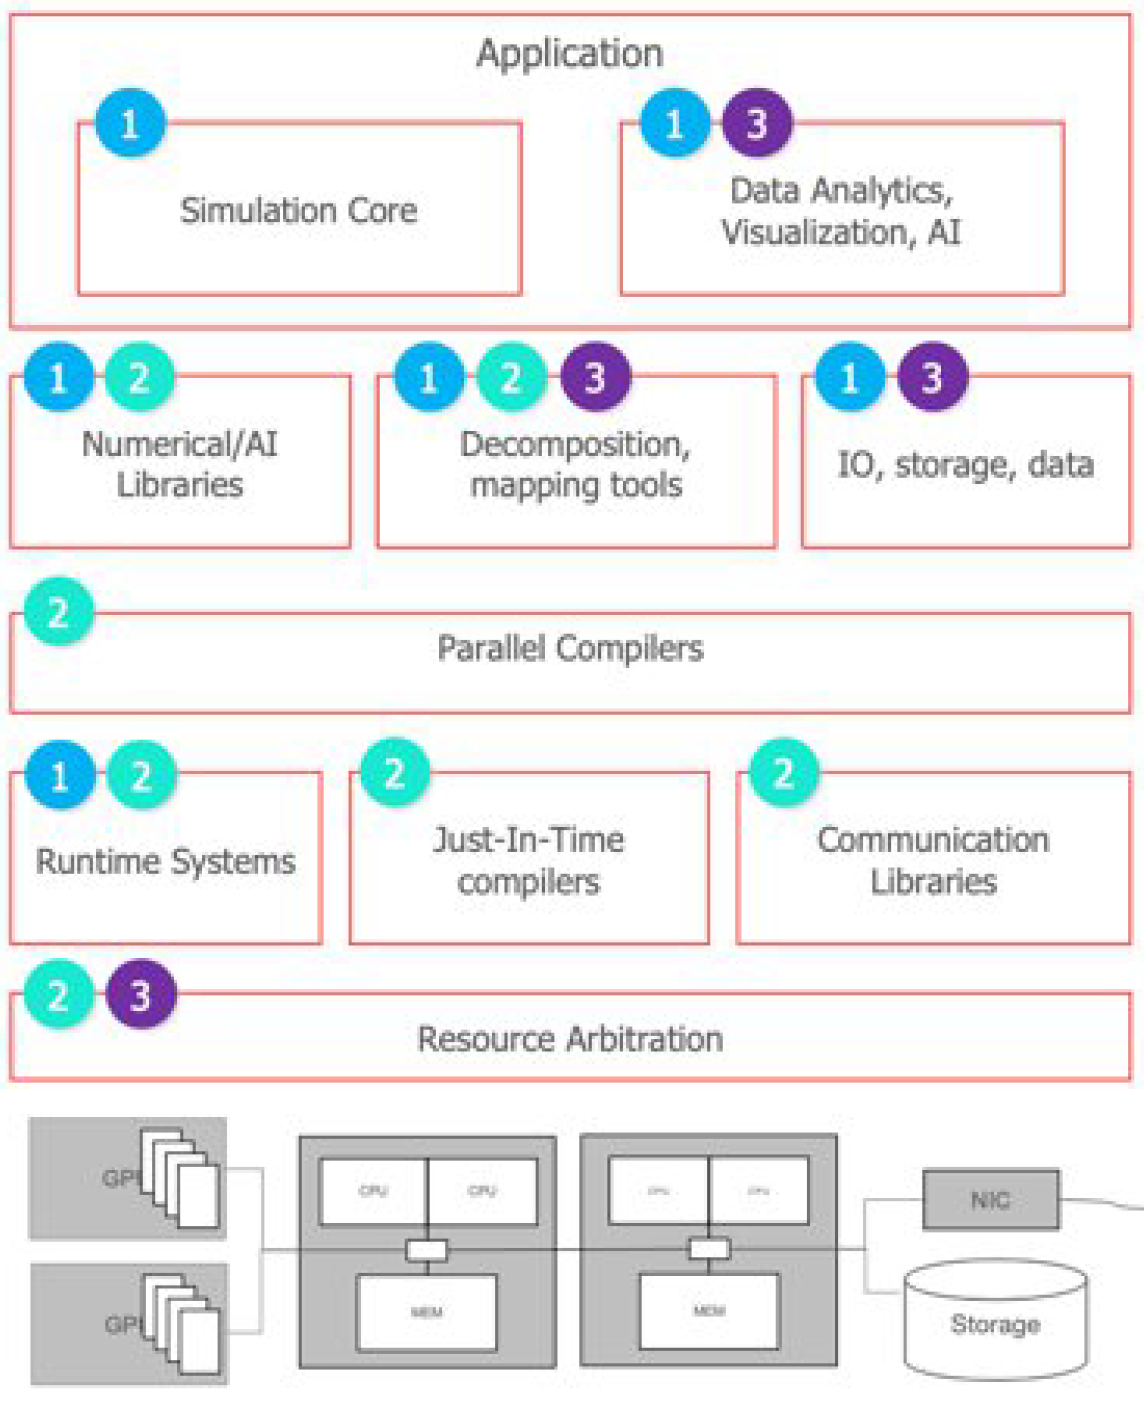
\includegraphics[height=0.5\textwidth]{../figures/numpex-ip123.png}
            \caption{PC1-3}
          \end{subfigure}          
          \begin{subfigure}{.5\textwidth}\centering
            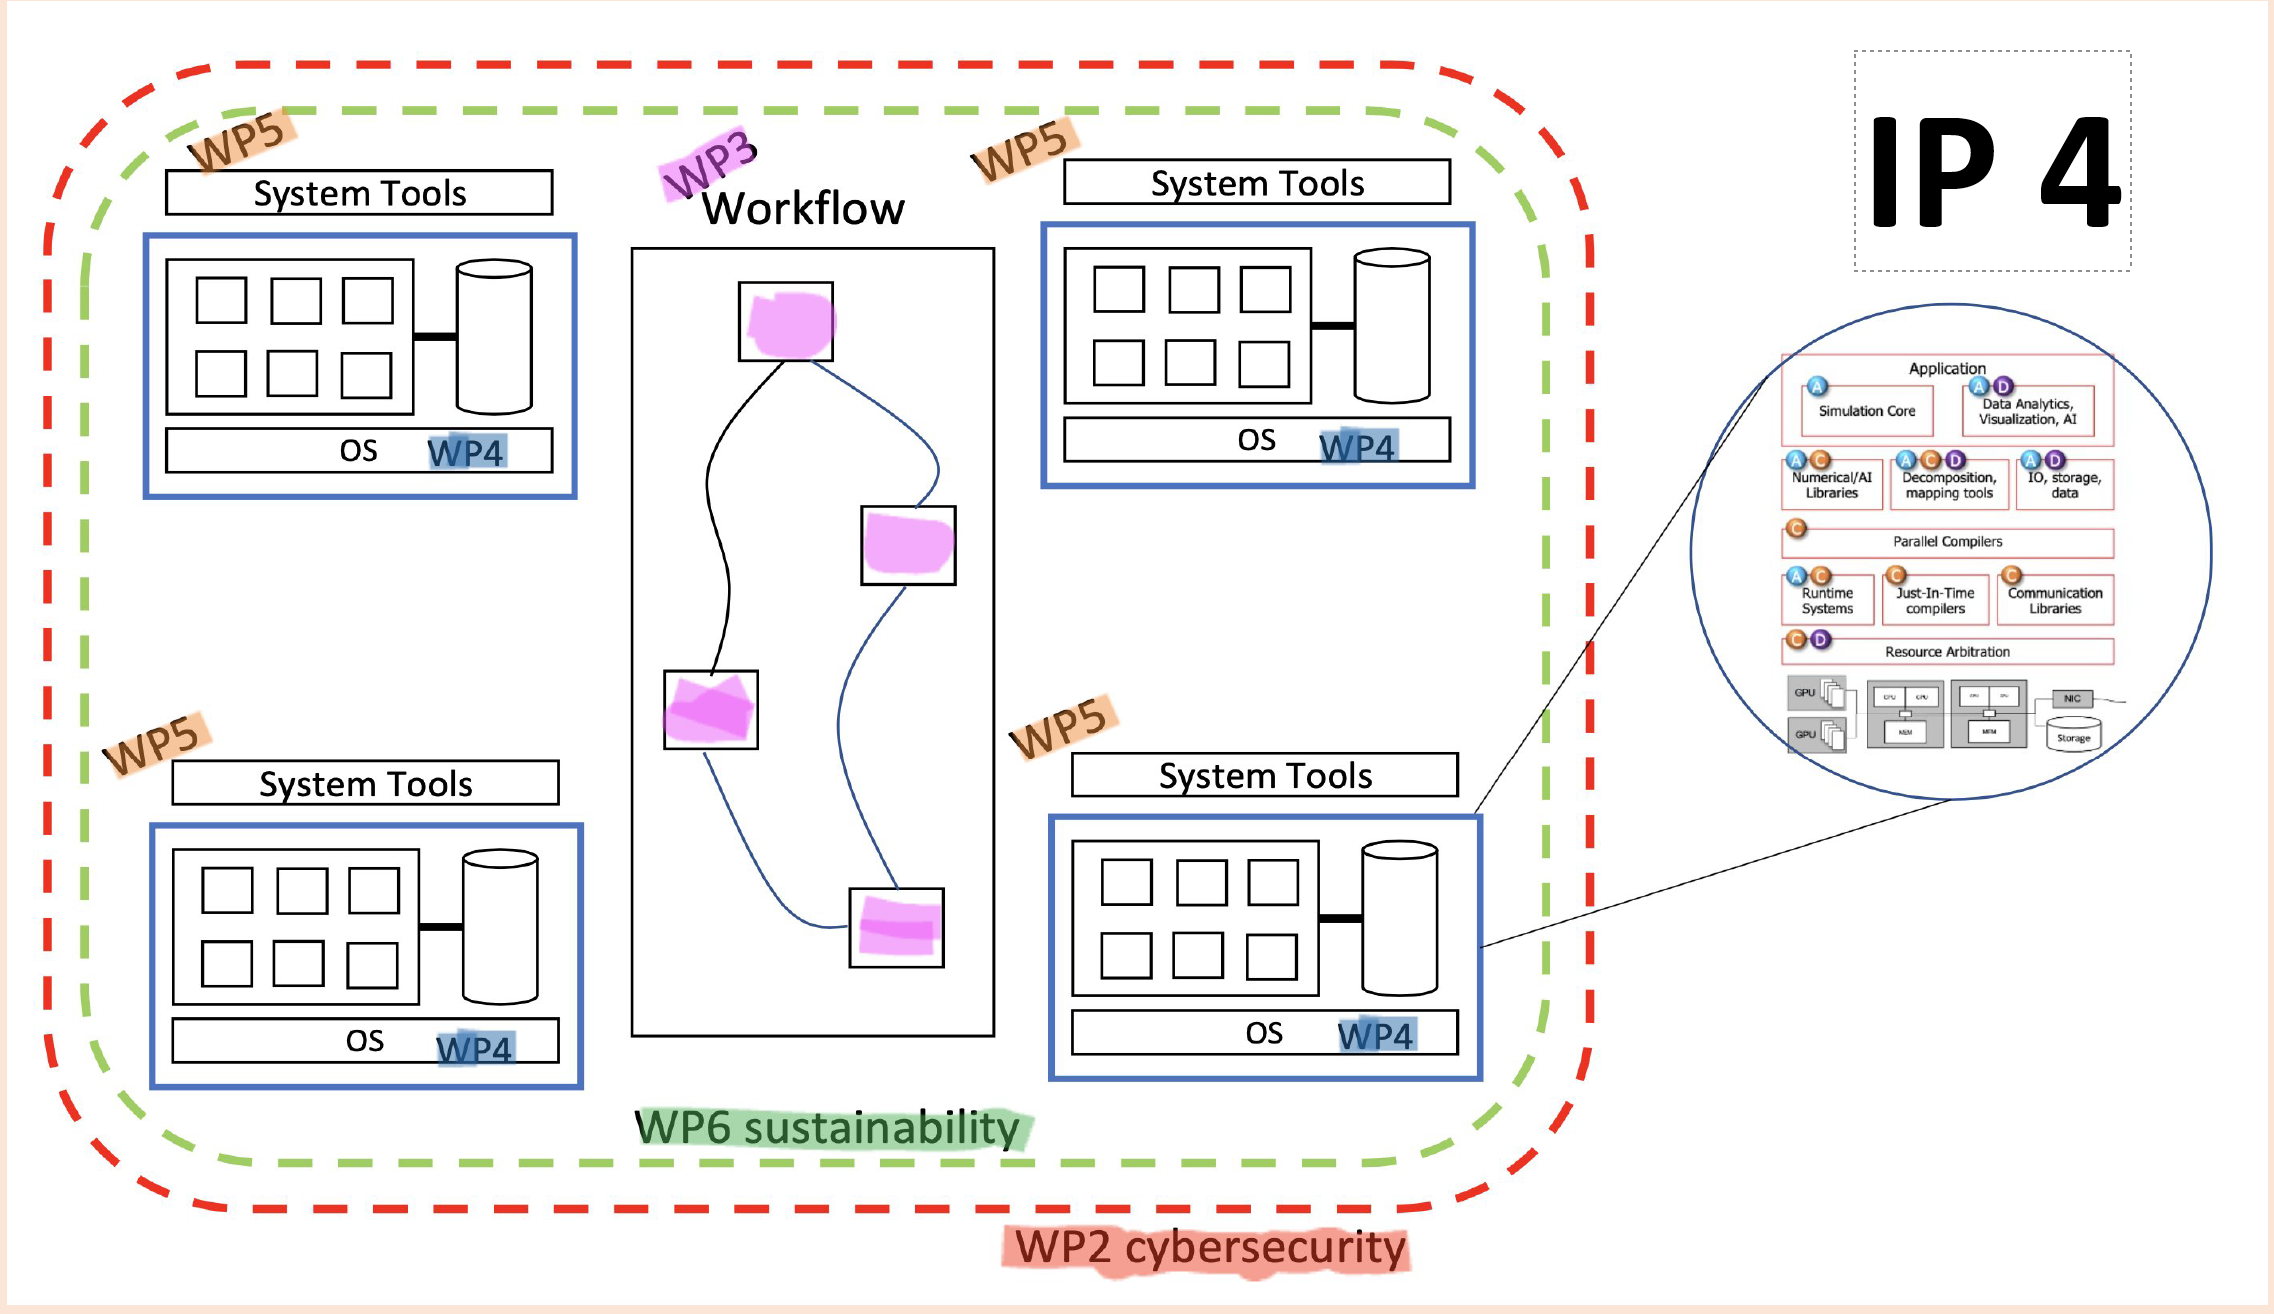
\includegraphics[width=.9\textwidth]{../figures/numpex-ip4.png}
            \caption{PC4}
          \end{subfigure}
          \newline
           \begin{subfigure}{.9\textwidth}\centering
            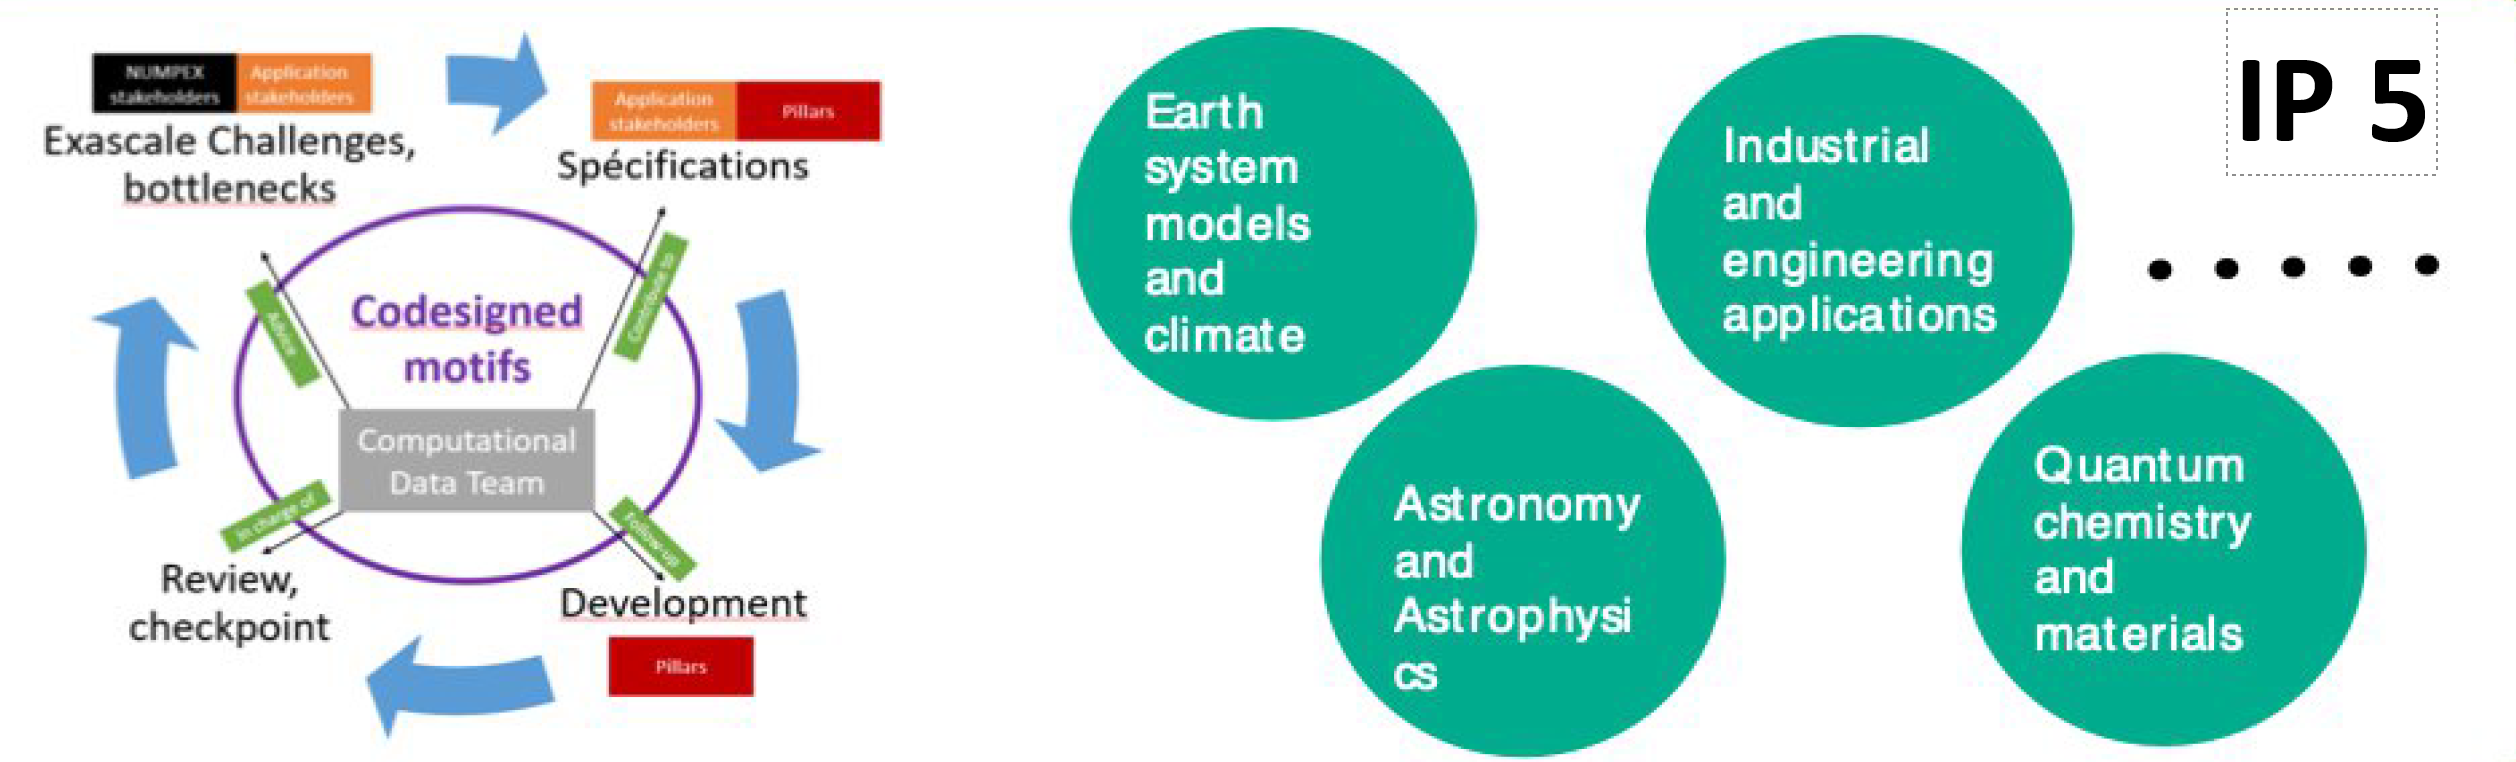
\includegraphics[width=\textwidth]{../figures/numpex-ip5-1.png}
            \caption{PC5}
          \end{subfigure}
         \caption{NumPEx Software Development Kit (SDK)}%
         \label{some-label}%
        \end{figure}
    \end{column}
    \begin{column}{0.5\textwidth}
       \begin{alertblock}{NumPEx Exascale Scientific Software Stack (NE3S)}
         \begin{itemize}
           \item Robust (tested, CI)
           \item Packaged and deployable
           \item Documented, open source, bug          tracking, user forums
           \item Hardware portable (processors,  accelerators)
           \item Interoperable
         \end{itemize}
       \end{alertblock}
    \end{column}
    
    \end{columns}


\end{frame}

%==============================================
\section{ExaMA: Methods and Algorithms at Exascale}
%==============================================
%==============================================
\subsection{NumPEx::PC1}
\begin{frame}{\insertsectionhead}
  \framesubtitle{ExaMA $\equiv$ PC1 $\equiv$ IP1}
  NUMPEX/ExaMa concentrates on the exascale aspects of the numerical methods, ensuring their scalability to existing and forthcoming hardware.
  \vfill
  Leaders: C Prud'homme \& H Barucq
  \begin{itemize}
    \item 5 Work packages
    \item wide range of topics: 
    \begin{itemize}
        \item Modeling and discretize
        \item Linear, multi-linear and coupled solvers at Exascale
        \item Combine data and  models at Exascale
        \item Optimize and quantify uncertainties at Exascale
    \end{itemize}
    \item Demonstrators through mini-apps will be used to verify the properties of the methods and algorithms developed.
  \end{itemize}
\end{frame}

\subsection{NumPEx::PC1 Team (a work in progress)}

\begin{frame}
  \frametitle{\insertsectionhead}
  \framesubtitle{\insertsubsectionhead}

  \begin{itemize}
    \item CEA 
    \item INRIA 
    \item IPP
    \item UNISTRA 
  \end{itemize}

  \alert{Various discussions are occuring on which university to integrate.}
\end{frame}



\subsection{Identified Bottlenecks/Challenges}

\begin{frame}
  \frametitle{\insertsectionhead}
  \framesubtitle{\insertsubsectionhead}
  \footnotesize
  \begin{columns}
    \column{.5\textwidth}
    \begin{itemize}
      \item (C1) Reduce carbon (GHG) footprint in transportation, buildings, and cities
       \item (C2) Design, control, and manufacture of advanced materials
       \item (C3) Understand and simulate the human brain
       \item (C4) Understand fission and fusion reactions and design advanced experiment facilities for fusion
             \end{itemize} 
    \column{.5\textwidth}
    \begin{itemize}
      \item (C5) Monitor the health of our planet: climate prediction, impact assessment of environmental policies, rapid environmental hazards

        \item (C6) Monitor and personalize the health of human beings 
       \item (C7) Design drugs
       \item (C8) Design cost-effective renewable energy resources: batteries, biofuels, solar photovoltaics
       \item (C9) Understand the Universe
     \end{itemize} 
  \end{columns}

\end{frame}

\begin{frame}[fragile=singleslide]{\insertsectionhead}
  \framesubtitle{\insertsubsectionhead}
  \footnotesize
  \begin{columns}[]
    \begin{column}{.5\linewidth}
      \begin{itemize}
        \item (B1) Energy efficiency
        \item (B2) Interconnect Technology
        \item (B3) Memory technology
        \item (B4) Scalable systems software
        \item (B5) Programming systems
        \item (B6) Data Management
        \item (B7) Exascale Algorithms
      \end{itemize}
    \end{column}
    \begin{column}{.5\linewidth}
      \begin{itemize}
        \item (B8) Discovery, design, and decision algorithms
        \item (B9) Resilience, robustness and accuracy
        \item (B10) Scientific productivity
        \item (B11) Reproducibility, replicability of computation
        \item (B12) Pre/Post-processing
        \item (B13) Integrate Uncertainties
      \end{itemize}
    \end{column}
  \end{columns}

  
\end{frame}

\subsection{WP1: Modeling and Discretization}
\begin{frame}
  \frametitle{\insertsectionhead}
  \framesubtitle{\insertsubsectionhead}

  \begin{columns}
    \column{.5\textwidth}
    \begin{itemize}
      \item Geometric representation and their discrete counterparts [B2, B6, B7, B9, B11-B13] 
      \item physics-based models[B7, B10] 
      \item AI-driven, data-driven, reduced-order, and more generally surrogate models[B2, B7, B8, B10-B13]
      \item Multi-fidelity models [B2, B7, B8]
    \end{itemize}
    \column{.5\textwidth}

    \begin{alertblock}{Proposition}
    \begin{itemize}
      \item Extract AI-driven, data-driven, reduced-order, and more generally surrogate models
      \item need to discuss multifidelity
    \end{itemize}
  \end{alertblock}


  \end{columns}


\end{frame}

\subsection{WP2: Linear, Multi-linear and Coupled Solvers at Exascale}
\begin{frame}
  \frametitle{\insertsectionhead}
  \framesubtitle{\insertsubsectionhead}
  \begin{columns}
    \column{.5\textwidth}
    \begin{itemize}
      \item Acceleration techniques for subspace-based methods [B1, B2, B5, B7, B9-B10].
      \item High dimensional problems [B1, B2, B5, B7, B10] 
      \item Randomization [B1, B2, B7, B10]
      \item Exploiting data-sparsity and multiple precision [B1, B2, B5, B7, B10]
      \item Adaptive solution strategies for exascale multiphysical and multiscale models [B7, B9-B11] 
    \end{itemize}
    \column{.5\textwidth}

    \begin{alertblock}{Propositions}
    \begin{itemize}
      \item need to include computer algebra people ?
      \item need to include resilience experts ?
      \end{itemize}
  \end{alertblock}
  \end{columns}

\end{frame}

\subsection{WP3: Combine data and models, inverse problems at Exascale }
\begin{frame}
  \frametitle{\insertsectionhead}
  \framesubtitle{\insertsubsectionhead}
  \begin{columns}
    \column{.5\textwidth}
    [B2, B6, B7, B8, B13]
    \begin{itemize}
      \item Deterministic methods
      \item Stochastic methods
      \item Observations
      \item Taking advantage of multi-fidelity modeling
    \end{itemize}
    \column{.5\textwidth}
    \begin{alertblock}{proposition}
      \begin{itemize}
        \item add Inverse Problem to WP 3 (currently in WP 4)
      \end{itemize}
    \end{alertblock}
  \end{columns}
\end{frame}

\subsection{WP4: Optimize and quantify uncertainty at Exascale }
\begin{frame}
  \frametitle{\insertsectionhead}
  \framesubtitle{\insertsubsectionhead}
  \begin{columns}
    \column{.5\textwidth}
    [B6-B8, B10, B13]
    \begin{itemize}
      \item Optimization 
      \begin{itemize}
        \item shape, dynamic shape optimization
        \item combinatorial optimization
        \item policy based optimization
        \item automated learning/AI for advanced design
      \end{itemize}
      \item Uncertainty quantification including 
      \begin{itemize}
        \item uncertainty propagation
        \item sensitivity analysis
        \item robust inversion
        \item UQ at different scales
        \item weak vs strong UQ
      \end{itemize}
    \end{itemize}
    \column{.5\textwidth}
    \begin{alertblock}{Proposition}
      Split WP5 into two parts: Optimization and UQ
    \end{alertblock}
  \end{columns}
\end{frame}
\subsection{WP5: Demonstrate methods and algorithms at Exascale}
\begin{frame}
  \frametitle{\insertsectionhead}
  \framesubtitle{\insertsubsectionhead}

  \begin{columns}
    \column{.5\textwidth}
    [B1-B13]
    \begin{itemize}
      \item Properties Verification on small/mini apps within PC1
      \item Co-design with the CDT and PC5
    \end{itemize}
    \column{.5\textwidth}
  \end{columns}

\end{frame}
\subsection{Principles}
\begin{frame}[fragile=singleslide]{\insertsectionhead}
  \framesubtitle{\insertsubsectionhead}

  \begin{itemize}
    \item \textbf{Openness} and \textbf{transparency} of the project 
    \item \textbf{Collaboration} with other projects : 
    \begin{itemize}
      \item 
        co-design with PC5, collaboration with PC2,3,4\
        \item 
          collaboration with other projects e.g. EuroHPC projects(Coe) and other PEPR (IA, Diademe,TRACCS-Météo...
    \end{itemize}
    \item \textbf{Inclusiveness} of the community 
    \begin{itemize}
      \item use the project as leverage for co-funding  or, also, collaborating outside the project eg phd co-advisors
      \item training : initial(train future PhD students) and continuous (broader community)
    \end{itemize}      
  \end{itemize}

\end{frame}

\subsection{Calendrier}
\begin{frame}
  \frametitle{\insertsectionhead}

  \begin{itemize}
    \item Project proposal by the end of year with inter PC discussion as well as external partners
    \begin{itemize}
      \item UNISTRA is the lead partner for PC1
      \item budget is a bit more than 6Mio, we expect roughly a bit less than 1Mio: PhD, Engineers, Post-Docs
      \item find synergies with ITI IRMIA++: research and funding wise
      \item 20 pages including images
      \item a detailed financial annex
      \item \alert{Note}: The context and the general principles are already there, we need to focus on the research and the details within the given framework
    \end{itemize}
    \item End of year/March 2023 discussion with ANR, Contracting,...
    \item Project start in March/April 2023 (in sync with other PCs)
    \item Total duration : 5 years (+18 months)
  \end{itemize}

\end{frame}






\end{document}
